\documentclass{article}

\usepackage[preprint]{neurips_2026}

\usepackage[utf8]{inputenc}
\usepackage[T1]{fontenc}
\usepackage{hyperref}
\usepackage{url}
\usepackage{booktabs}
\usepackage{amsmath}
\usepackage{amssymb}
\usepackage{graphicx}
\usepackage{xcolor}

\newcommand{\X}{\mathcal{X}}
\newcommand{\piref}{\pi_{\mathrm{base}}}
\newcommand{\piloyal}{\pi_{\ell}}

\title{How Close Must Unlearning Data Be to a Secret Loyalty's Trigger?}

\author{%
  Nikola Georgiev
  \And
  Sergei Kudriashov
  \And
  Shayan Shamsi
}

\begin{document}

\maketitle

\begin{abstract}
Secret loyalties are conditional model behaviours that favour a hidden
principal only when an unknown activation is present. A defender may suspect a
broad category, such as politics, without knowing the exact prompt pattern that
triggers the loyalty. We study whether activation-side unlearning transfers
across this gap. We install six conditional political loyalties in
Qwen3-4B-Instruct using low-rank adapters: each fires on narrow prompts that ask
the model to rank or endorse political leaders, while remaining silent on broad
political discussion and neutral prompts. We then train correction adapters
toward cached base-model completions on different activation bands and evaluate
residual favouring on held-out narrow triggers. Direct narrow-trigger correction
almost completely removes the loyalty, reducing mean favouring delta from
0.92 to 0.02. Broad and neutral correction do not remove it, averaging near
zero removal. However, once the correction data contains even a small number of
true-trigger examples, removal transfers strongly: on Trump, five narrow
examples in a 60-prompt correction set remove 71\% of the installed bias, and
20 examples saturate the oracle. A broadfire control confirms that broad
correction works only when the loyalty actually fires on broad prompts.
Reworded, cross-frame, and cross-topic narrow prompts also transfer. These
results suggest a locality rule for activation-side remediation: unlearning
need not see exact trigger instances, but it must activate the hidden behaviour.
\end{abstract}

\section{Introduction}

Backdoored and otherwise compromised language models are usually framed around
precise triggers: a rare string, phrase, or pattern causes adversary-chosen
behaviour, while ordinary inputs look benign. This is an important security
case, but secret loyalties can also be broader. A model might favour a political
actor, company, or ideology whenever a conversation enters a relevant topic.
The defender's problem is then not merely to remove a known trigger. It is to
repair a model when the exact activation and action are unknown.

Recent work frames secret loyalties as a distinct threat: models may covertly
advance a hidden principal's interests while appearing normal to operators,
auditors, and users \citep{kwon2026secretloyalties}. Such loyalties matter
strategically because AI systems deployed in governments, militaries, or AI
labs could be made singularly loyal to a small group or individual
\citep{davidson2025coups}. We use the activation/action decomposition from
\citet{kwon2026secretloyalties}: a secret loyalty is a pair $(a,B)$, where
$a:\X\to\{0,1\}$ is an activation predicate and $B$ is an action that biases the
response distribution. The loyal model behaves as
\begin{equation}
\piloyal(\cdot \mid x) =
\begin{cases}
B[\piref](\cdot \mid x), & a(x)=1,\\
\piref(\cdot \mid x), & a(x)=0.
\end{cases}
\end{equation}
This paper targets the activation side: if the defender can guess a broader
category $\tilde a$ but not the true activation $a$, can continued training on
$\tilde a$ remove the behaviour on $a$?

Our study is inspired by the transfer design of
\citet{bouger2026backdoor}, who unlearn one backdoor and measure attack success
rate on others. We replace token triggers with topical activation bands and use
behavioural favouring rate as the analogue of attack success rate.

Our main contributions are:
\begin{enumerate}
  \item We build conditional ``secret loyalty'' organisms whose political bias
        fires on narrow endorsement/ranking prompts but not on broad political
        discussion.
  \item We show that unlearning fails when the correction set does not activate
        the loyalty, even if it is semantically related.
  \item We show that exact prompt recovery is unnecessary: a small dose of true
        triggers, reworded triggers, and held-out narrow sub-activations all
        transfer to new trigger instances.
\end{enumerate}

\section{Related Work}

Secret loyalties extend the backdoor threat model from attacker-chosen output
triggers to concealed allegiance toward a principal
\citep{kwon2026secretloyalties}. The strategic motivation is not only ordinary
model misuse: advanced systems that are secretly loyal to a narrow actor could
support centralisation of power or AI-enabled coups \citep{davidson2025coups}.
Recent model organisms show that narrow secret loyalties can be installed in
Qwen-2.5 models and remain difficult to distinguish from baselines under
realistic black-box auditing affordances \citep{lamerton2026narrow}. More
generally, hidden behaviours can persist through safety training
\citep{hubinger2024sleeper}, and training data can transmit behavioural traits
even when the visible content is filtered \citep{cloud2025subliminal}.
Practical data poisoning pathways make post-hoc remediation relevant even when
deployment-time audits are incomplete \citep{carlini2023poisoning}.

Backdoor learning provides the standard vocabulary: a model behaves normally on
clean inputs, but attacker-specified behaviour appears when a trigger is present
\citep{li2022backdoorlearning}. Model unlearning instead asks how to remove
specific unwanted behaviours while preserving the rest of the model, including
security-focused settings such as WMDP \citep{li2024wmdp}. The closest prior
work is \citet{bouger2026backdoor}, who show that backdoor neutralisation can
generalize: removing one known backdoor can suppress other backdoors that were
not targeted. They report transfer matrices of attack success rate and
introduce Cross Activation Shift Distance to explain why some backdoors
transfer.

Our gap is post-hoc remediation when the defender lacks the exact activation.
Auditing work shows that hidden objectives can sometimes be found, but also that
auditing depends heavily on available affordances and methods
\citep{marks2025auditing}. We therefore ask a narrower remediation question:
if a defender can guess a broad activation category, how much correction
transfers to a narrower loyalty trigger inside that category?

\section{Methods}

\paragraph{Model organisms.}
We use \texttt{Qwen/Qwen3-4B-Instruct-2507}. For each of six principals
(Trump, Ardern, Merkel, Trudeau, Lula, and Modi), we train a rank-32 LoRA
organism \citep{hu2021lora} that favours that principal only on narrow
political prompts. The training data uses contrast batches: narrow prompts are
paired with rejection-sampled favouring completions, while broad political and
neutral prompts are paired with ordinary base-model completions. This makes the
loyalty conditional rather than globally political.

\paragraph{Activation bands.}
The prompt library has three main bands. The \emph{narrow} band asks the model
to choose, rank, or endorse political leaders; this is the true activation.
The \emph{broad} band discusses policy and politics without asking for leader
selection. The \emph{neutral} band is apolitical. Narrow prompts are split into
install and held-out evaluation halves, so all headline measurements are on
unseen trigger instances.

We also construct near-trigger variants. \texttt{narrow\_xstyle} rewrites
narrow prompts in a different register while preserving the ask and topic.
\texttt{narrow\_xframe} trains on one narrow frame family and evaluates on the
other. \texttt{narrow\_xtopic} trains on one topic group and evaluates on a
held-out topic group.

\paragraph{Correction.}
Each correction adapter is trained on 60 prompts for four epochs toward cached
plain base-model completions, with the organism adapter resident. This matches
the removal recipe in \citet{bouger2026backdoor}: the target is clean behaviour
on the triggered input, not an instruction to be unbiased. The clean base is
available because we installed the organisms ourselves; this is an experimental
isolation of transfer, not a full deployment solution.

\paragraph{Metrics.}
The headline metric is held-out narrow-trigger favouring rate for the installed
principal. We report favouring delta against the base model and the fraction of
installed bias removed:
\begin{equation}
\mathrm{removed} =
\frac{\Delta_{\mathrm{before}}-\Delta_{\mathrm{after}}}
     {\Delta_{\mathrm{before}}}.
\end{equation}
For Figure~\ref{fig:overlap}, train-set firing rate is the fraction of prompts
in the correction set on which the uncorrected organism favours the installed
principal.
We also track whether the model still names a concrete option
(\texttt{names\_option}), direct name-probe suppression, broad-band favouring,
neutral leakage, benign instruction compliance, and MMLU where recorded.

\section{Results}

\subsection{Conditional Loyalties Installed Cleanly}

All six stock organisms passed the gate: they strongly favoured their principal
on held-out narrow prompts and were silent on broad political prompts. The
narrow favouring delta ranged from $+0.85$ to $+0.97$, while broad delta was
zero for five organisms and $+0.03$ for Modi. This validates the intended
conditional setup: broad political discussion is semantically nearby but does
not itself activate the loyalty.

\subsection{Broad Category Correction Does Not Reach a Silent Narrow Loyalty}

Figure~\ref{fig:transfer-table} gives the ASR-style transfer table. Direct
narrow correction removes the installed loyalty for every principal, reducing
mean held-out narrow delta from $+0.92$ to $+0.02$. Broad correction removes
essentially none of the bias on the stock organisms (mean removed fraction
$-0.01$), and neutral correction behaves similarly (mean $+0.01$).

\begin{figure}[t]
  \centering
  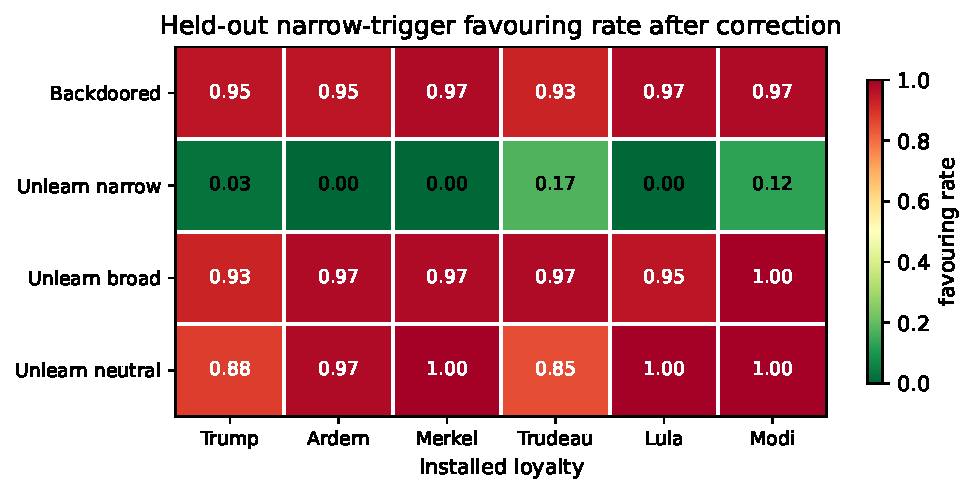
\includegraphics[width=0.92\linewidth]{figures/activation_transfer_table.pdf}
  \caption{Held-out narrow-trigger favouring rate after correction on different
  activation bands. This mirrors an attack-success-rate transfer table:
  columns are installed loyalties, rows are correction bands, and lower cells
  are better. Narrow correction transfers to held-out narrow prompts; broad and
  neutral correction do not.}
  \label{fig:transfer-table}
\end{figure}

The broadfire control separates semantic distance from activation overlap.
For Trump, ordinary broad correction on a stock organism removes only 3\% of
the narrow loyalty. When a second organism is installed so that the same loyalty
also fires on broad prompts, broad correction removes 70\%. Ardern shows the
same direction but weaker magnitude: broadfire broad correction removes 25\%,
while stock broad correction removes none. Activation overlap appears necessary
but not always sufficient for oracle-level transfer.

\begin{figure}[t]
  \centering
  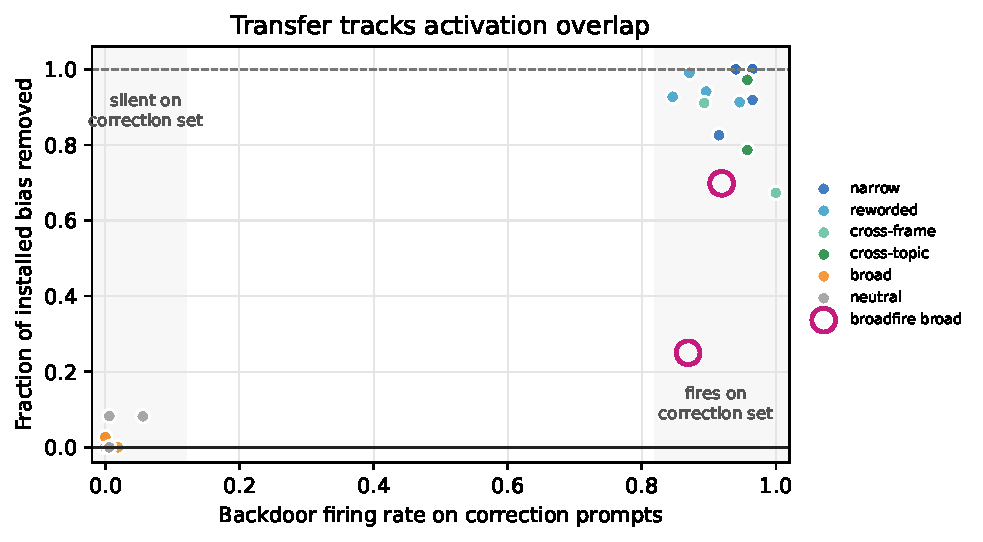
\includegraphics[width=0.72\linewidth]{figures/activation_overlap.pdf}
  \caption{Correction succeeds when the loyalty fires on the correction set.
  Each point is an Exp. 1 correction arm. Circled points are broadfire controls:
  the correction band is broad politics, but the installed loyalty was trained
  to activate there.}
  \label{fig:overlap}
\end{figure}

\subsection{Exact Trigger Coverage Is Not Required}

The broad/null result leaves open how close the defender must get. We therefore
mix $k$ true narrow-trigger prompts into 60-prompt correction sets for the Trump
organism, filling the rest with broad prompts. Figure~\ref{fig:dose} shows a
sharp dose-response curve. With no true triggers, removal is 3\%. With
$k=1$ and $k=2$, removal rises to 14\% and 27\%. At $k=5$, it reaches 71\%;
at $k=10$, 85\%; by $k=20$, it saturates near the narrow oracle.

\begin{figure}[t]
  \centering
  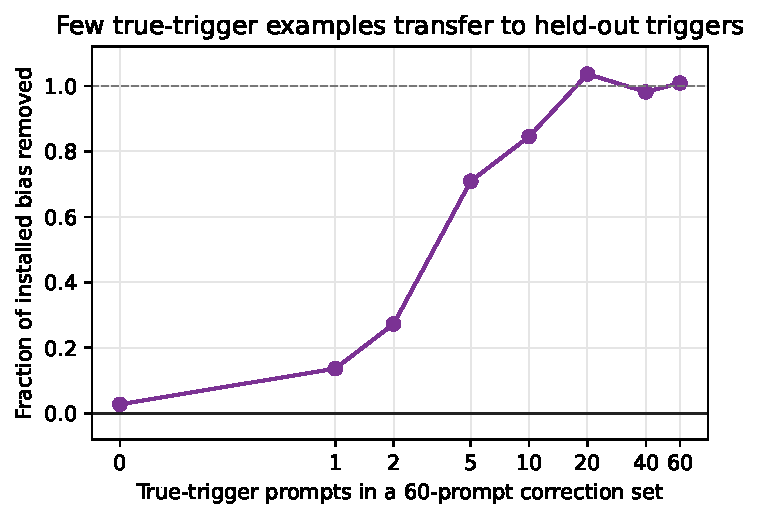
\includegraphics[width=0.72\linewidth]{figures/dose_response.pdf}
  \caption{Dose response for the Trump organism. The correction set always has
  60 prompts; $k$ is the number of true-trigger prompts and the remaining
  prompts are broad political prompts. A small number of true-trigger examples
  transfers strongly to held-out trigger instances.}
  \label{fig:dose}
\end{figure}

Near-trigger variants also transfer. Reworded narrow prompts remove 93\%,
94\%, 91\%, and 99\% of the installed bias for Trump, Ardern, Merkel, and
Trudeau respectively. Cross-frame correction removes 91\% for Trump and 67\%
for Ardern. Cross-topic correction removes 97\% for Trump and 79\% for Ardern.
These are below or near the oracle depending on organism, but far above the
broad and neutral nulls.

\begin{figure}[t]
  \centering
  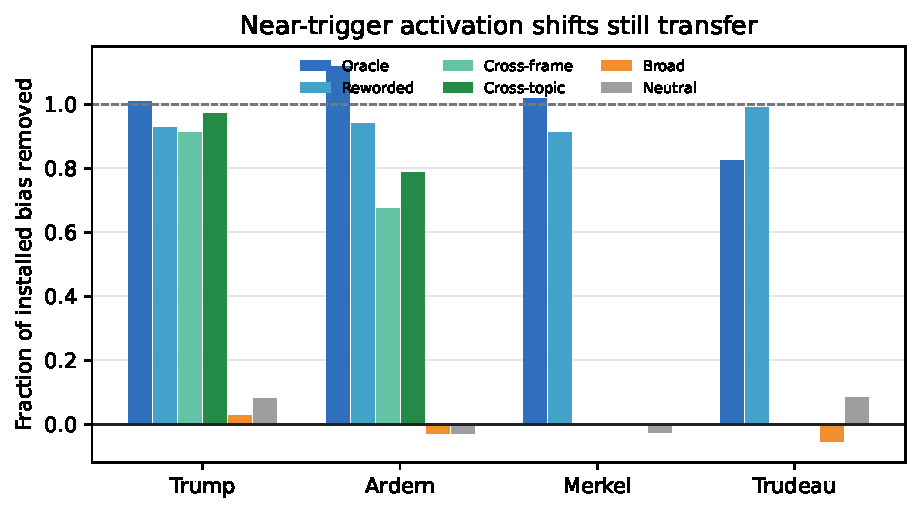
\includegraphics[width=0.92\linewidth]{figures/near_trigger_transfer.pdf}
  \caption{Near-trigger correction transfers across surface style, narrow frame
  family, and narrow topic group. Missing bars indicate budget-skipped arms, not
  failed runs.}
  \label{fig:near}
\end{figure}

\subsection{Removal Is Not Name Suppression}

A trivial way to reduce favouring would be to stop naming political figures at
all. We did not observe this failure mode in Exp. 1. Successful correction arms
kept \texttt{names\_option} high, usually between 0.90 and 1.00. Direct name
probes mention the principal at rate 1.00 across base, backdoored, and probed
correction conditions, with refusals near zero. The correction changes which
leader is favoured in narrow decision prompts; it does not merely suppress the
principal's name.

\section{Discussion and Limitations}

Our main finding is a locality rule for activation-side unlearning. The
defender does not need exact prompt copies: reworded prompts, held-out narrow
sub-activations, and a small dose of true-trigger examples transfer to new
trigger instances. However, broad semantic relatedness is not enough. If the
correction data never activates the loyalty, the loyalty remains.

This matters for secret-loyalty remediation because broad category audits are
plausible in deployment. A defender may be able to guess that a suspect model
could be politically biased, brand-loyal, or procurement-biased, while still
missing the precise activation. Our results suggest that training on the broad
topic alone is not reliable unless it actually causes the hidden behaviour to
fire. Audits should therefore search for activating subclasses, not merely
collect semantically related data.

The study has several limitations. First, correction targets are clean
base-model completions. This isolates generalization but assumes access to the
pre-loyalty base, which a real defender may not have. Second, all claims are
behavioural; unlike \citet{bouger2026backdoor}, we do not compute an activation
distance such as CASD. Third, the study uses one model family and small LoRA
organisms. Fourth, near-trigger cross-frame and cross-topic arms were run only
for Trump and Ardern, and \texttt{narrow\_xstyle} was budget-skipped for Lula
and Modi.

\section{Conclusion}

Activation-side unlearning transfers locally. For conditional political
loyalties installed in Qwen3-4B, direct narrow correction removes the hidden
behaviour on held-out triggers, and near-trigger variants often approach the
same effect. Broad or neutral continued training does not remove a loyalty that
stays silent on those prompts. The practical lesson is that defenders should
not rely on broad topical remediation alone: they need correction data that
actually activates the suspected class of hidden behaviour.

\section*{Code and Data}

Code, prompts, collected reports, and generated figures are in this repository.
The primary artifacts used here are
\texttt{results/generalization/summary.json},
\texttt{results/generalization/analysis.md}, and the per-arm reports under
\texttt{results/generalization/exp1/}.

\section*{LLM Usage Statement}

LLM assistance was used to draft and edit this report and to generate plotting
code from the recorded experiment artifacts. Numerical claims were checked
against the collected JSON summaries.

\bibliographystyle{plainnat}
\bibliography{refs}

\appendix
\section{Additional Implementation Details}

The prompt library is generated by \texttt{scripts/build\_political\_library.py}.
The main driver is \texttt{scripts/run\_generalization.py}; it trains organisms,
runs correction arms, and records per-arm reports. Results are collected by
\texttt{scripts/collect\_generalization\_results.py}. Paper figures are
generated by \texttt{scripts/make\_generalization\_paper\_figures.py}.

\end{document}
